\documentclass[../main.tex]
		
		\begin{document}
			\section{Functions}
	\begin{description}
		\item[Task:] Define a function rigorously and make sense of terminology associated to functions.
		\item[Definition:] Let $A, B$ be sets. A function $f:A \rightarrow B$ is a rule that assigns to \underline{every} element of $A$ \underline{one and only one} elements of $B$, \textbf{i.e.} $\forall x \in A \exists! y \in B$ s.t. $f(x)=y$. $A$ is called the \underline{domain} of $f$ and $B$ is called the \underline{codomain}.
		\item[Examples:]
		\begin{enumerate}
			\item[]
			\item $A = \{1, 3, 7\}$ \\
			$B = \{1, 2, 5\}$
			\begin{figure}[h]
				\centering
				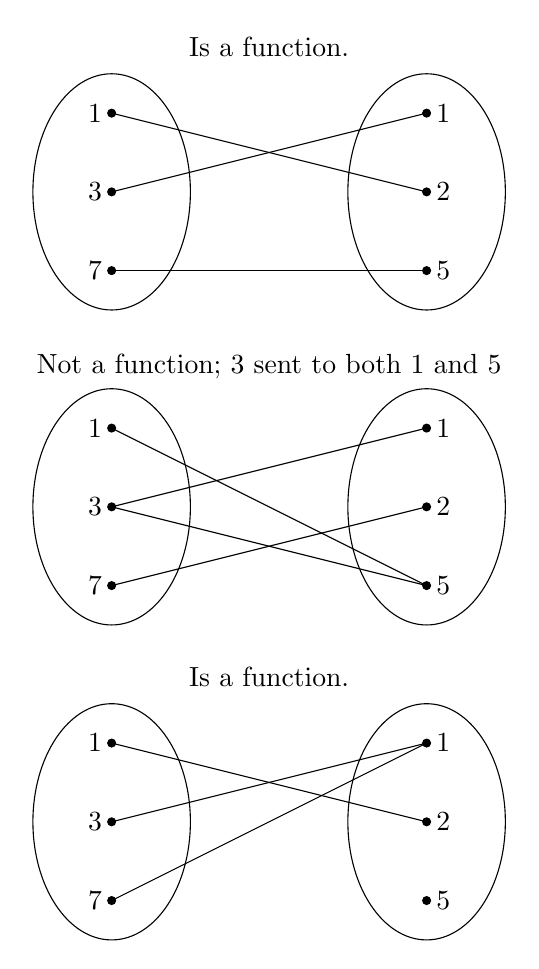
\begin{tikzpicture}	
					\begin{scope}
						\draw (0, 1.6) node[above] {Is a function.};
						\coordinate (A1) at (-2, 1);
						\coordinate (A2) at (-2, 0);
						\coordinate (A3) at (-2, -1);
					
						\draw (A1) node[left]{1};
						\draw (A2) node[left]{3};
						\draw (A3) node[left]{7};
						\draw[fill=black] (A1) circle(0.5mm);
						\draw[fill=black] (A2) circle(0.5mm);
						\draw[fill=black] (A3) circle(0.5mm);
						
						\coordinate (B1) at (2, 1);
						\coordinate (B2) at (2, 0);
						\coordinate (B3) at (2, -1);
						
						\draw (B1) node[right]{1};
						\draw (B2) node[right]{2};
						\draw (B3) node[right]{5};
						\draw[fill=black] (B1) circle(0.5mm);
						\draw[fill=black] (B2) circle(0.5mm);
						\draw[fill=black] (B3) circle(0.5mm);
						
						\draw (-2, 0) circle [x radius=1, y radius=1.5];
						\draw (2, 0) circle [x radius=1, y radius=1.5];
						
						\draw (A1) -- (B2);
						\draw (A2) -- (B1);
						\draw (A3) -- (B3);
					\end{scope}
					
					\begin{scope}[yshift=-4cm]
						\draw (0, 1.5) node[above] {Not a function; 3 sent to both 1 and 5};
						\coordinate (A1) at (-2, 1);
						\coordinate (A2) at (-2, 0);
						\coordinate (A3) at (-2, -1);
					
						\draw (A1) node[left]{1};
						\draw (A2) node[left]{3};
						\draw (A3) node[left]{7};
						\draw[fill=black] (A1) circle(0.5mm);
						\draw[fill=black] (A2) circle(0.5mm);
						\draw[fill=black] (A3) circle(0.5mm);
						
						\coordinate (B1) at (2, 1);
						\coordinate (B2) at (2, 0);
						\coordinate (B3) at (2, -1);
						
						\draw (B1) node[right]{1};
						\draw (B2) node[right]{2};
						\draw (B3) node[right]{5};
						\draw[fill=black] (B1) circle(0.5mm);
						\draw[fill=black] (B2) circle(0.5mm);
						\draw[fill=black] (B3) circle(0.5mm);
						
						\draw (-2, 0) circle [x radius=1, y radius=1.5];
						\draw (2, 0) circle [x radius=1, y radius=1.5];
						
						\draw (A1) -- (B3);
						\draw (A2) -- (B1);
						\draw (A2) -- (B3);
						\draw (A3) -- (B2);
					\end{scope}
					
					\begin{scope}[yshift=-8cm]
						\draw (0, 1.6) node[above] {Is a function.};
						\coordinate (A1) at (-2, 1);
						\coordinate (A2) at (-2, 0);
						\coordinate (A3) at (-2, -1);
										
						\draw (A1) node[left]{1};
						\draw (A2) node[left]{3};
						\draw (A3) node[left]{7};
						\draw[fill=black] (A1) circle(0.5mm);
						\draw[fill=black] (A2) circle(0.5mm);
						\draw[fill=black] (A3) circle(0.5mm);
										
						\coordinate (B1) at (2, 1);
						\coordinate (B2) at (2, 0);
						\coordinate (B3) at (2, -1);
										
						\draw (B1) node[right]{1};
						\draw (B2) node[right]{2};
						\draw (B3) node[right]{5};
						\draw[fill=black] (B1) circle(0.5mm);
						\draw[fill=black] (B2) circle(0.5mm);
						\draw[fill=black] (B3) circle(0.5mm);
										
						\draw (-2, 0) circle [x radius=1, y radius=1.5];
						\draw (2, 0) circle [x radius=1, y radius=1.5];
										
						\draw (A1) -- (B2);
						\draw (A2) -- (B1);
						\draw (A3) -- (B1);
					\end{scope}
				\end{tikzpicture}
			\end{figure}
			\item $A=B=\mathbb{R} \hspace{10mm} F:\mathbb{R} \rightarrow \mathbb{R}$ given by $f(x)=x$ is called the identity function.
		\end{enumerate}
		\item[Definition:] Let $A, B$ be sets and let $f: A \rightarrow B$ be a function. The \underline{range} of $f$ denoted by $f(A)$ is the subset of $B$ defined by $f(A) = \{y \in B \mid \exists x \in A$ s.t. $f(x)=y \}$.
		\item[Definition:] Let $A$ be a set. A \underline{Boolean function} on $A$ is a function $F:A \rightarrow \{T, F\}$ which has $A$ as its domain and the set of truth values $\{T, F\}$ as is codomain. $f:A \rightarrow \{T, F\}$ thus assigns truth values to the elements of $A$.
	\end{description}
	Function are often represented by graphs. If $f:A \rightarrow B$ is a function, the \underline{graph} of $f$ denoted $\Gamma (f)$ is the subset of the Cartesian product $A \times B$ given by $\{(x, f(x)) \mid x \in A \}.$
	\begin{description}
		\item[Q:] Is it possible to obtain every subset of $A \times B$ as the graph of some function?
		\item[A:] No! For $f:A \rightarrow B$ to be a function $\forall x \in A \hspace{5mm} \exists! y \in B$ s.t. $f(x)=y$, so for $\Gamma \subseteq A \times B$ to be the graph of some function, $\Gamma$ must satisfy that $\forall x \in A \hspace{5mm} \exists! y \in B$ s.t. $(x, y) \in \Gamma$. Then we can define $f$ by letting $y = f(x)$.
	\end{description}
	

\end{document}